%Adaptive sparse quadrature forward UQ on reduced dimensional space.
By this stage, the parameters that contribute most to the uncertainty
have been reduced to a more manageable number, so that a global
examination can be made of this remainder.
Relevant techniques employed during this stage are
\begin{itemize}
\item Sparse quadrature sampling, especially adaptive
\item Forward UQ
\item Sobol Analysis
%\item PGD
\end{itemize}

\subsubsection{Sparse Quadrature Sampling}\label{sec:sparse}
The idea of sampling on sparse grids seems to have supplanted QMC sampling (see Appendix~\Sec{QMC})
for many applications, presumably because it can be made to adapt to the functional
dependence of outputs suggested by the sampling, unlike QMC or indeed Latin hypercube sampling (see Appendix~\Sec{LHSamp}).
The review article~\cite{Bu04Spar} is remarkable for the wide range of references
on the subject of sparse sampling, not just in application to quadrature (evaluating integrals
of functions). The key idea is best illustrated graphically,
see \Fig{sgridl}, and is that provided the integrand is well behaved,
it is sufficient to have sample or quadrature points concentrated along
the coordinate axes in the centre of the domain.
(There is a variant which includes samples at the edge of the
domain of integration.)
\begin{figure}
\centerline{\rotatebox{0}{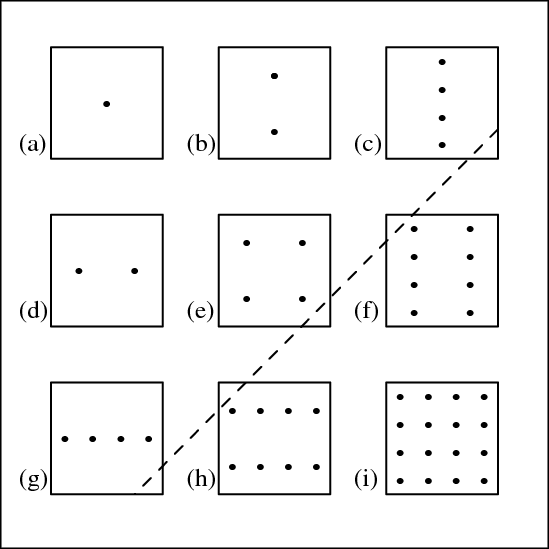
\includegraphics[width=9.5cm]{../png/sgridl}}}
\caption{\label{fig:sgridl}
Sparse grid sampling. The point sets lying below the diagonal drawn dashed
are omitted.}
\end{figure}
The resulting set of sample points is shown in \Fig{stog}(a). The
locations of the points in the higher order sets are always determined
by bisecting the positions of those in the lower order sets.

Provided that integrands are sufficiently smooth,
integrals can be proved~\cite{Bu04Spar} to converge at a rate
\begin{equation}\label{eq:sparsec}
\mathcal{O}(\log(N)^{d-1}/N)
\end{equation}
where $d$ is the number of dimensions over which the integral is performed.
Indeed, by careful choice of point sets, excluding some which
lie above the equivalent of the diagonal in \Fig{sgridl} for
greater sampling density than shown there,
it is possible to achieve convergence of the integral at a rate
\begin{equation}\label{eq:sparsen}
\mathcal{O}(N^{-1})
\end{equation}
There is the important caveat that this rate is achieved only in
the `energy' norm:
\begin{equation}\label{eq:ennorm}
\parallel Q \parallel_E = \sqrt{\left(\int \sum_{i=1}^d \left(\frac{\partial Q}{\partial x_i}\right)^2 d{\mathbf x}\right)}
\end{equation}
and in other norms the $d$-dependent rate \Eq{sparsec} is found. Nonetheless
this implies that the number of samples needed to characterise the
parameter space is
\begin{equation}\label{eq:nsparsec}
\mathcal{O}(N \log(N)^{d-1})
\end{equation}

\begin{figure}
\centerline{
\rotatebox{0}{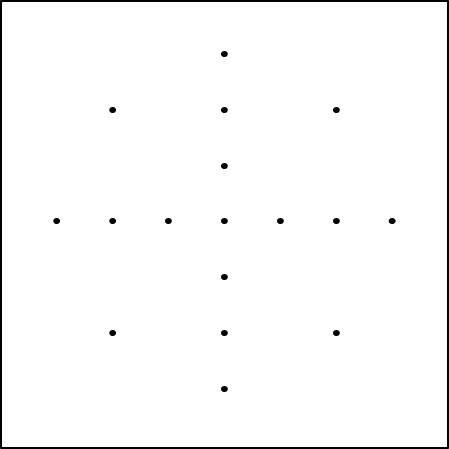
\includegraphics[width=5.5cm]{../png/stogsym}}
\rotatebox{0}{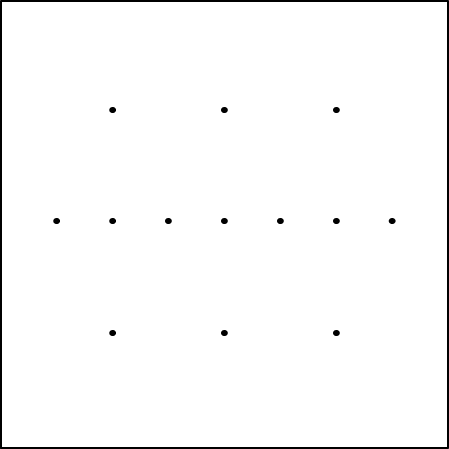
\includegraphics[width=5.5cm]{../png/stog}}
}
\caption{\label{fig:stog}
On the left is an example of isotropic sparse grid sampling.
The diagram on the right indicates how the vertical direction may
be more coarsely sampled than the horizontal, by omitting further
the point set labelled~(c) in \Fig{sgridl}.}
\end{figure}
If singularities are present, then sparse grids can be locally
adapted~\cite[end \S\,4]{Bu04Spar}, most easily using the fact their
construction by bisection naturally leads to error estimates
based on the difference between the solutions on the mesh
before and after subdivision.
As explained in ref~\cite{Ge03Dime} sparse
grids can also be dimension adaptive, placing more points in
some coordinate directions than others, as illustrated in the right diagram of \Fig{stog}.

\subsubsection{Forward UQ}\label{sec:forward}
``Forward UQ" is conceptually the easiest kind of uncertainty quantification,
in that it is assumed that the uncertainties are known at the outset. Thus in the case
of a physics-based problem, all the important physical processes are regarded
as having been identified, so that they can be parameterised. These parameters will 
in turn have known uncertainties, specified via probability distributions denoted $p(x)$.

The commonest distribution is the Gaussian, as a consequence of the Central
Limit Theorem, which states that the probability
distribution for the sum of an increasing number of independently and identically
distributed random variables with appropriately normalised finite mean and variance tends
to the ``Normal" (ie.\ Gaussian) distribution. In practice the theorem is found to apply
to most measurements, implying it is accurate for numbers less than ten,
as the measurement chain from
experiment to observer typically involves the compounding of a relatively small number of errors.
If parameters are expressed in terms of bounds on their extreme values,
this of course corresponds to uniform distributions. ``Interval analysis"~\cite{Pa15Unce}
includes this case, but also the Dempster-Shafer structure, whereby
uncertainty is described by overlapping parameter intervals with different
uniform probabilities.

It is straightforward, given a random number generator~(RNG) that is equally likely
to return any number~$\xi_i$ within the unit interval~$[0,1]$
to scale the outputs to be uniformly distributed
in an arbitrary finite interval~$[a,b]$, and relatively
straightforward to arrange so that numbers are output with a given frequency
distribution. Both commercial (such as matlab$^{TM}$) and opensource packages
(eg.\ Python NumPy Generator~\cite{numpyrandwebsite}) are available.
They rely on the fact that the
cumulant (ie.\ definite integral) of a probability distribution is uniformly
distributed, so that if the Cumulant~$P(x)$ is defined as
\begin{equation}\label{eq:cumul}
P(x)=\int_{-\infty}^x  p(x') dx'
\end{equation}
then samples~$x_i= P^{-1}(\xi_i), i=1,2,\ldots, N$ become distributed according to~$p(x)$
as $N$~becomes large.

Forward UQ most easily proceeds by constructing an ensemble of realisations of the 
detailed models at parameters sampled according the specified distributions.
A distribution for each QoI may be estimated using the ensemble, from which
follows an average and a standard deviation estimate for the QoI.
Thus it is customary to talk of uncertainty as being propagated through the system.

%``Forward UQ" should be contrasted with Inverse UQ, where the aim is to estimate the
%distribution describing the uncertainties in the parameters given an ensemble of data.

\subsubsection{Sobol}\label{sec:sobol}

The use of adaptive sparse grids is a well-established procedure, see ref~\cite{He03Adap}
to perform the Sobol ANOVA-like analysis.
The approach described by Sobol~\cite{So01Glob} (based on a Russian paper from~1990)
is based on a function-theoretic result which applies
to a function which must at least be continuous.
The `Sobol' decomposition generalises ANOVA, where ANOVA stands for `Analysis
of Variance', a family of statistical methods for quantifying how the outputs
of a system depend on its inputs, usually based on linearity assumptions.

Suppose that the function is $f\left(\mathbf{x}\right)=f\left(x_1,x_2,\dots,x_d\right)$
where ${\mathbf x} \in I^d$ (i.e.\ $0 \leq x_k \leq 1, k=1, \dots, d$), then the Sobol decomposition is
\begin{equation}\label{eq:fexp}
f\left(x_1,\ldots,x_d\right)=f_0+\sum_{k=1}^d f_k\left(x_k\right)+\sum_{j=1}^{d-1}\sum_{k=j+1}^d f_{jk}\left(x_j,x_k\right)+ \cdots +f_{12 \dots d}({\mathbf x})
\end{equation}
where $f_0$ is a constant and the integral of each term in the sums is zero, i.e.
\begin{equation}\label{eq:fint}
\int_0^1 f_{j_1 j_2 \dots j_r}\left(x_{j_1},x_{j_2},\dots,x_{j_r}\right)dx_{j_k}=0, \;\;\; 1 \leq k \leq r
\end{equation}
There is the expectation that this latter property ensures that the
term of higher order in~$r$ become negligible. The applicability to statistical
analysis is evident when it is realised that \Eq{fexp}  may be interpreted as an expansion for the joint
probability distribution~$f\left(x_1,\ldots,x_d\right)$
since, integrating over the variables~$x_{j_r}$ as appropriate and using \Eq{fint} gives
\begin{eqnarray}\label{eq:effe}
f_0&=&\mathbb{E}(f) \nonumber \\
f_i(x_i)&=&\mathbb{E}(f|x_i)-f_0 \label{eq:effe1}\\
f_{ij}(x_i,x_j)&=&\mathbb{E}(f|x_i,x_j)-f_0-f_i(x_i)-f_j(x_j) \label{eq:effe2}
\end{eqnarray}
so that the numbered equations give successively the effect of variation of one variable,
two-way interactions, etc. Similarly, squaring \Eq{fexp} and integrating gives
relations for the variances
\begin{eqnarray}\label{eq:sens}
V_i(x_i)&=&\mathrm{Var}_{x_i}\left(\mathbb{E}_{x_{k\neq i}}(f|x_i)\right) \\
V_{ij}(x_i,x_j)&=&\mathrm{Var}_{x_{ij}}\left(\mathbb{E}_{k\neq i, l\neq j}(f|x_i,x_j)\right)-V_i-V_j  \label{eq:sens2}
\end{eqnarray}
($k\neq i$ denotes that the expectation~$\mathbb{E}$ is computed by integrating over all the $x_k$ except for~$x_i$)
which normalised by the variance~$\mathrm{Var}(f)$ are equal to the Sobol sensitivity indices
$S_i$, $S_{ij}$, \ldots, respectively.

As noted by Huan~et~al~\cite[\S\,3.2]{Hu18Glob}, the Sobol indices may be expressed directly as sums of
squares of the coefficients of a PCE. It will be evident that $S_i$~gives a normalised measure
of the sensitivity of the distribution of~$f$ to the parameter~$x_i$, so that small~$S_i$
justifies neglect of $x_i$ in subsequent analysis.
